% !TeX root = Protokoll.tex
% !TeX root = ../../.global/latex/preamble.tex
\subsection{Magnetische Momente}
Ein Elektron im Atom besitzt zu einem den Bahndrehimpuls $\vec{l}$ und zum anderen wie ein Eigendrehimpuls fungierenden Spin $\vec{s}$.
Die Beträge dieser vektoriellen Größen werden bestimmt durch
\begin{align}
	|\vec{l}|=&\sqrt{l(l+1)}\hbar\\
	\nonumber &\text{und}\\
	|\vec{s}|=&\sqrt{s(s+1)}\hbar.
\end{align}
Dabei sind $l$ und $s$ die Quantenzahlen, sowie $\hbar$ das Plancksche Wirkungsquantum.
Aufgrund der Ladung der Elektronen, entsteht da durch magnetische Momente $\vec{\mu_l}$ und $\vec{\mu_s}$ .
Mithilfe des Bohrschen Magnetons 
\begin{align}
	\mu_B:=-\frac{1}{2}e_0 \frac{\hbar}{m_0},
\end{align}
lassen sich diese Momente berechnen durch
\begin{align}
	\vec{\mu}_l=&-\mu_B\sqrt{l(l+1)}\vec{e}_l\\
	\nonumber &\text{und}\\
	\vec{\mu}_s=&-g_s\,\mu_B\sqrt{s(s+1)}\vec{e}_s.
\end{align}
Hier sind ist $e_0$ die Elementarladung, $m_0$ die Elektronmasse.
Weiter wird für $\vec{\mu}_s$ der Landé-Faktor eingeführt, der die Stärke der der Kopplung des Spins ans magnetische Moment beschreibt.\\
Für Atome mit mehr als ein Elektron gibt es verschiedene Arten, wie der Bahndrehimpulse und der Spin wechselwirken können.
Grundlegend werde zwei grundlegenden Fälle unterschieden.
Zum einen für Atome mit niedriger Kernladungszahl und zum anderen mit hoher.
Bei Atomen mit kleiner Kernladungszahl, ist die Wechselwirkungen den Drehimpulsen groß.
Deshalb lässt sich ein Gesamtdrehimpuls definieren als
\begin{align}
	\vec{L}:=\sum_i \vec{l}_i\, \text{ mit }\, |\vec{L}|=\sqrt{L(L+1)}\hbar.
\end{align}
Weil der Drehimpuls abgeschlossener Schalen immer Null ist, reicht es über die Drehimpulse der der nicht abgeschlossenen Schalen zu summieren.
Es treten nur Gesamtdrehimpulse auf, deren Quantenzahl ganzzahlig ist.
Dabei werden den Quantenzahlen L=0, 1, 2 oder 3 den Termen S, P, D oder F zugewiesen.\\
Zu dem Gesamtbahndrehimpuls lässt sich ein magnetisches Moment $\vec{\mu}_L$ aufstellen als
\begin{align}
	|\vec{\mu}_L|=\mu_B\sqrt{L(L+1}).
\end{align}
Es lässt sich weiter ein Gesamtspin $\vec{S}$ definieren als
\begin{align}
	\vec{S}=\sum_is_i \text{ mit } |\vec{S}|=\sqrt{S(S+1)}\hbar.
\end{align}
Für die Gesamtspinquantenzahl gilt $S=\frac{N}{2},\ \frac{N}{2}-1 ,\ \dots,\ \frac{1}{2},\ 0$, wobei $N$ die Anzahl der Elektronen der nicht abgeschlossenen Schale ist.
Das magnetische Moment das durch den Gesamtspin hervorgerufen wird, lässt sich mit
\begin{align}
	|\vec{\mu}_S|=g_S\ \mu_B\sqrt{S(S+1)}
\end{align}
berechnen.
Bei nicht zu großen externen Magnetfeldern lässt sich der Gesamtdrehimpuls bestimmen als
\begin{align}
	\vec{J}=\vec{L}+\vec{S} \ \text{ mit }\ |\vec{J}|=\sqrt{J(J+1)}\hbar.
\end{align}
Ein Energie Niveau kann mithilfe von 
\begin{align}
	{}^M\mathcal{L}_J
\end{align}
ausgedrückt werden.
Darin Bezeichnet $M=2S+1$ und $\mathcal{L}\in\{S|L=0,\ P|L=1,\ D|L=2,\ F|L=3\}$ referiert zu der Quantenzahlen des Bahndrehimpulses.
Diese Art der Kopplung wird LS-Kopplung genannt.\\
Der Zweite Fall, der mit Großer Kernladungszahl, wird j-j-Kopplung genannt.
Hier koppelt der Spin und der Bahndrehimpuls eines Elektrons stark, gegenüber den Anteilen der anderen Elektronen.
Dadurch addieren sich der Spin und der Bahndrehimpuls zum Gesamtdrehimpuls des Elektrons, so dass 
\begin{align}
	\vec{j}_i=\vec{l}_i+\vec{s}_i
\end{align}
gilt.
Dann lässt sich der Gesamtdrehimpuls des Atoms schreiben als
\begin{align}
	\vec{J}=\sum_i\vec{j}_i,
\end{align}
allerdings existieren keine Gesamtbahndrehimpulse bzw. Gesamtspins.
Zwischen diesen Beiden Grenzfällen herrscht ein fließender Übergang.\\
Zu dem Gesamtdrehimpuls lässt sich ein magnetisches Moment berechnen als
\begin{align}
	\vec{\mu}_J&=\mu_Bg_J\sqrt{J(J+1)},
\end{align}
wobei gilt
\begin{align}
		g_J:=&\frac{3J(J+1)+S(S+1)-L(L+1)}{2J(J+1)}.
\end{align}
Dabei wird $g_J$ als Landé-Faktor des entsprechenden Atoms bezeichnet.
\subsection{Energieaufspaltung und Übergänge}
\begin{figure}[h!]
	\centering
	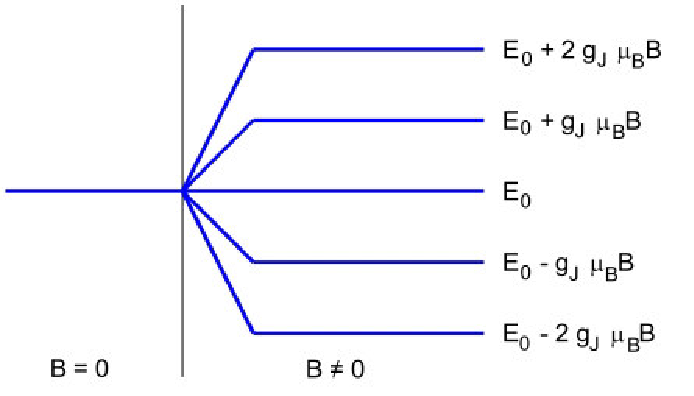
\includegraphics[width=0.6\textwidth]{../Grafiken/fig_theo_Aufspaltung.pdf}
	\caption{Aufspaltung eines Energieniveaus von einem Atoms mit $J=2$. \cite{V27}}\label{fig:Theo_Aufspaltung}
\end{figure}
\noindent
Wird an einem Atom mit Gesamtdrehimpuls $\vec{J}$ ein Homogenes Magnetfeld $\vec{B}$ angelegt, so ist die resultierende Energie 
\begin{align}
	E_\text{mag}= -\vec{\mu}_J\cdot\vec{B}=mg_J\mu_B,
\end{align}
wobei $m$ die Richtungsquantelung ist, für die gilt $-J\le m\le J$.
Dies gilt weil nur bestimmte Winkel zwischen dem Magnetfeld und dem magnetischen Moment auftreten, sodass die $z$-Komponente ein vielfaches von $g_J\mu_B$ ist.
Es tritt dem nach eine Aufspaltung in $2J+1$ Niveaus auf, dies ist anhand des Beispiels $J=2$ in \cref{fig:Theo_Aufspaltung} dargestellt.\\
Die Übergänge der Energie Niveaus wird mithilfe der zeitabhängigen Schrödingergleichung beschrieben
\begin{align}
	\frac{\hbar^2}{2m}\Delta \psi(\vec{r},t)+U\psi(\vec{r},t)-i\hbar\frac{\partial \psi(\vec{r},t)}{\partial t}=0.
\end{align}
Dabei soll $\psi$ zwei Energieniveaus $\alpha$ und $\beta$ beschreiben.
Zwischen ihnen soll mit der Frequenz 
\begin{align}
	\nu_{\alpha\beta}:=\frac{E_\alpha-E_\beta}{h}
\end{align}
oszilliert werden.
Daraus lässt sich erkennen, dass das Elektron einen Dipol beschreibt. 
Das Dipolmoment in $x$-Richtung kann mithilfe von
\begin{align}
	D_x=-e_0\text{const}\real\left( \underbrace{\int x\psi^*_\beta\psi_\alpha dV}_{X_{\alpha\beta}}\exp(2\pi i\nu_{\alpha\beta}t) \right),
\end{align}
ausgedrückt werden.
Analog können die Komponenten für die $y$ und $z$-Richtung aufgestellt werden.
Die Matrixelemente $Z_{\alpha\beta}$, $X_{\alpha\beta}\pm i Y_{\alpha\beta}$ verschwinden, es sei den es gilt
\begin{align}
	\Delta m = m_\alpha-m_\beta = 0,\pm1
\end{align}
Aus der Konstruktion der Matrixelemente kann sich überlegt werden, dass bei $\Delta m=0$ ($Z_{\alpha\beta}\not=0,\ X_{\alpha\beta}\pm i Y_{\alpha\beta}=0$) der Dipol entlang der Magnetfeldachse schwingt und Strahlt somit linear-polarisiertes Licht Parallel zum Magnetfeld, diese Strahlungsart wird mit einem $\pi$ gekennzeichnet.
Für $\Delta m =\pm1$ gilt $Z_{\alpha\beta}=0$ und $\ X_{\alpha\beta}\pm i Y_{\alpha\beta}\not=0$, daraus lässt sich schließen, dass entweder links oder rechts zirkular-polarisiertes Emission um das Magnetfeld auftritt, diese wird als $\sigma$-Emission bezeichnet.\\
Die Überlegungen gelten für den Fall $S=0$, dabei wird vom normalen Zeeman-Effekt geredet.
Bei Übergängen mit $S=0$ gilt $g_J=1$.
Bei dem anormalen Zeeman-Effekt verschwindet die Spinquantenzahl nicht.
Hier bei gelten die selben Auswahlregeln für $\Delta m=0,\pm1$.
Allerdings ist nicht mehr $g_J=1$ gegeben, deshalb ist es Sinnvoll die Energie der Spektrallinie zu definieren
\begin{align}
	E=\underbrace{(m_ig_{J_i}-m_jg_{J_j)}}_{g_{ij}}\mu_BB+E_0=g_{ij}\mu_BB+E_0.
\end{align}
Darin ist $g_{ij}$ der Landé-Faktor des Übergangs.
\subsection{Übergänge der Cd-Lampe}
In diesem Versuch werden die Übergänge Einer Cd-Lampe untersucht.
Deshalb ist es von Interesse diese Übergänge genauer zu untersuchen.
Hier werden zwei Spektrallinien untersucht.
Erstens eine rote mit einer Wellenlänge von $\SI{643,8}{\nano\meter}$ die durch den Übergang ${}^1P_1\leftrightarrow{}^1D_2$ hervorgerufen wird.
Als Zweites wird eine Blaue betrachtet mit einer Wellenlänge von $\SI{480}{\nano\meter}$ die durch den Übergang ${}^1S_1\leftrightarrow{}^3P_1$ ausgelöst. 
Die Termschema sind in \cref{fig:termschema_rot} und \cref{fig:termschema_blau} dargestellt, die dazugehörigen Landé-Faktoren werden in \cref{tab:Lande_rot} und \cref{tab:Lande_blau} berechnet.
Dabei entspricht die rote Spektrallinie den anormalen Zeeman-Effekt und die blaue dem normalen Zeeman-Effekt.
%\subsection{Vorbereitungaufgaben}

\FloatBarrier
\begin{figure}[!h]
\centering
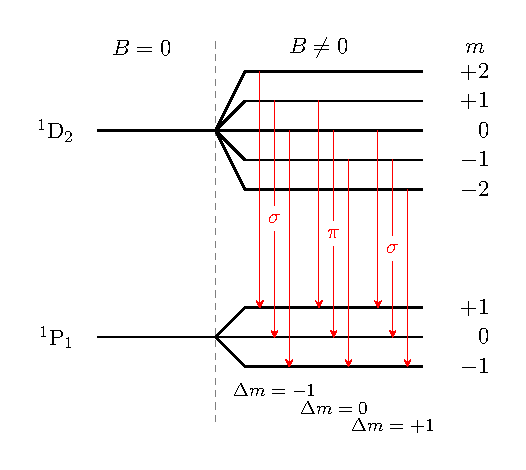
\includegraphics[scale=1.15]{../Grafiken/termschema_rot.pdf}
\caption{Hier ist das Termschema der roten Spektrallinie einer Cd-Lampe dargestellt\label{fig:termschema_rot}}
\end{figure}
\FloatBarrier
\FloatBarrier
\begin{figure}[!h]
\centering
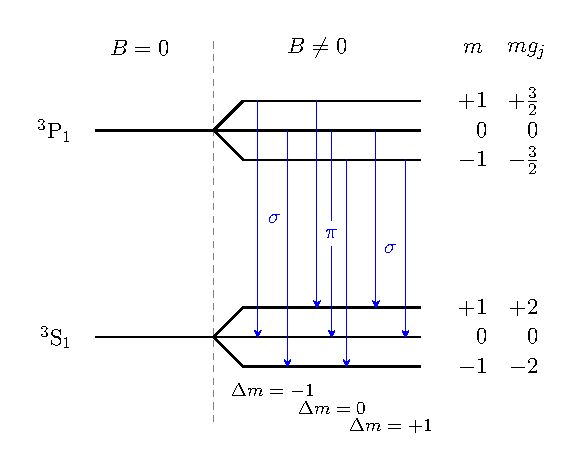
\includegraphics[scale=1.25]{../Grafiken/termschema_blau.pdf}
\caption{\label{fig:termschema_blau}}
\end{figure}
\FloatBarrier

\begin{table}
	\centering
	\begin{tabular}{cccccc}
		\toprule
		Übergang & $m_1$  & $g_{1}$ & $m_2$ & $ g_2$ & $g_{12}$\\
		\midrule
		& \multicolumn{2}{c}{${}^1P_1$}  & \multicolumn{2}{c}{${}^1D_2$} \\
		\midrule
		& 2 & 1 & 1 & 1 & 1\\
		$\sigma$& 1 & 1 & 0 & 1 & 1\\
		& 0 & 1 & -1 & 1 & 1\\
		\midrule
		& 1 & 1 & 1 & 1 & 0\\
		$\pi$ & 0 & 1 & 0 & 1 & 0\\
		& -1 & 1 & -1 & 1 & 0\\
		\midrule
		& 0 & 1 & 1 & 1 & -1\\
		$\sigma$ & -1 & 1 & 0 & 1 & -1\\
		& -2 & 1 & -1 & 1 & -1\\\bottomrule
	\end{tabular}
	\caption{Hier sind die Landé-Faktoren der roten Spektrallinie aufgeführt.}
	\label{tab:Lande_rot}
\end{table}
\begin{table}
	\centering
	\begin{tabular}{cccccc}
		\toprule
		Übergang & $m_1$  & $g_{1}$ & $m_2$ & $ g_2$ & $g_{12}$\\
		\midrule
		& \multicolumn{2}{c}{${}^3S_1$}  & \multicolumn{2}{c}{${}^3P_2$} \\
		\midrule
		$\sigma$ & +1 & 2 & 0 & $\frac{3}{2}$& 2\\
		& 0 & 2 & -1 & $\frac{3}{2}$ & $\frac{3}{2}$\\
		\midrule
		& +1 & 2 & +1 & $\frac{3}{2}$ & $\frac{1}{2}$\\
		$\pi$ & 2 & 2 & 0 & $\frac{3}{2}$ & 0 \\
		& -1 & 2 & -1 & $\frac{3}{2}$ & -$\frac{1}{2}$\\
		\midrule
		& 0 & 2 & 1 & $\frac{3}{2}$ & -$\frac{3}{2}$\\
		$\sigma$ & -1 & 2 & 0 & $\frac{3}{2}$& -2\\
		\bottomrule
	\end{tabular}
	\caption{Hier sind die Landé-Faktoren der blauen Spektrallinie aufgeführt.}
	\label{tab:Lande_blau}
\end{table}